{
\usebackgroundtemplate{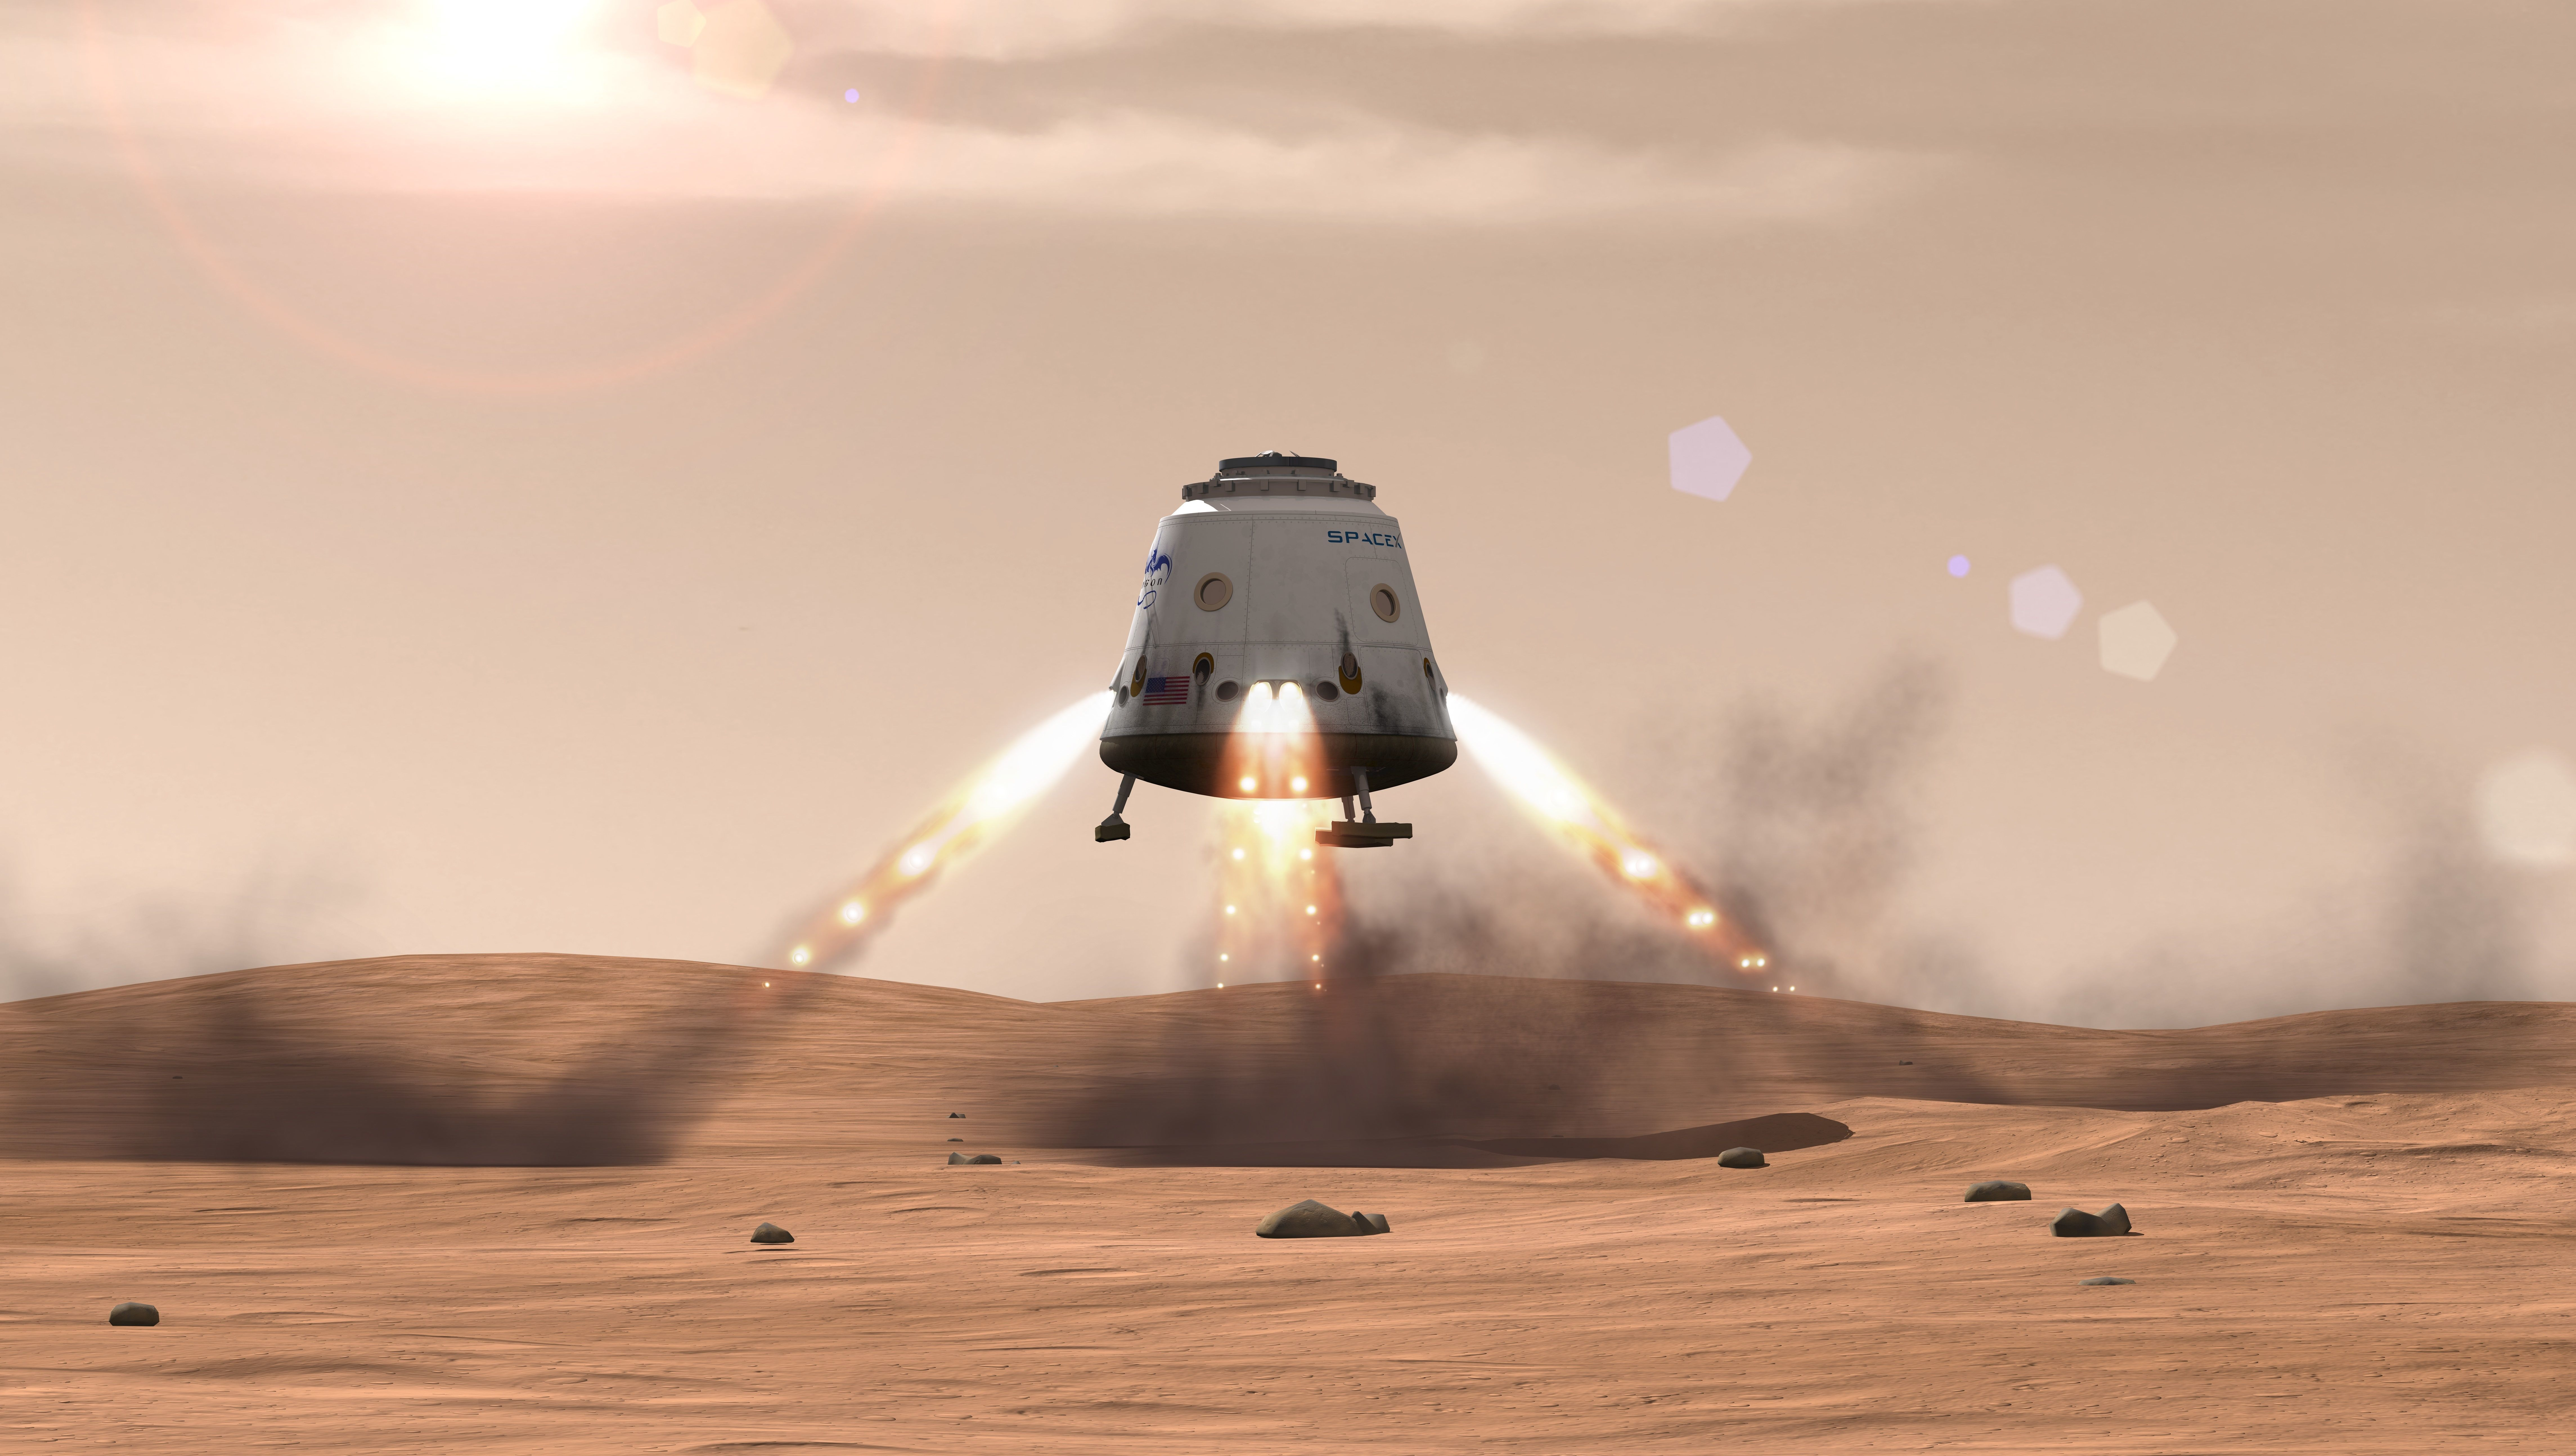
\includegraphics[height=\paperheight, keepaspectratio]{images/landing}}%
\begin{frame}
\end{frame}
\begin{frame}[t]{Landing}
    \begin{block}{Entering atmosphere}
        \begin{itemize}
            \item determine entry angle
            \item not to steep $=>$ to much atmosperic drag $=>$ burning up
            \item not to shallow $=>$ won't slow down quickly enough $=>$ skipping out of atmosphere
        \end{itemize}
    \end{block}
\end{frame}
\begin{frame}[t]{Landing}
    \begin{block}{Suicide Burn}
        We need to slow down our descent before we hit the ground. At the last possible second we fire all engines at 100\% throttle.
    \end{block}
    \begin{block}{Why?}
        \begin{itemize}
            \item Gravity is an accelerating force adding $\alpha m/s^2$
            \item Every second spend descelarating needs to be compensated for gravity
            \item Slowing down means burning an additional $\alpha$ delta-v every second
            \item Slowing down quickly saves fuel.
        \end{itemize}
    \end{block}
\end{frame}
}
\begin{frame}[t]{}
    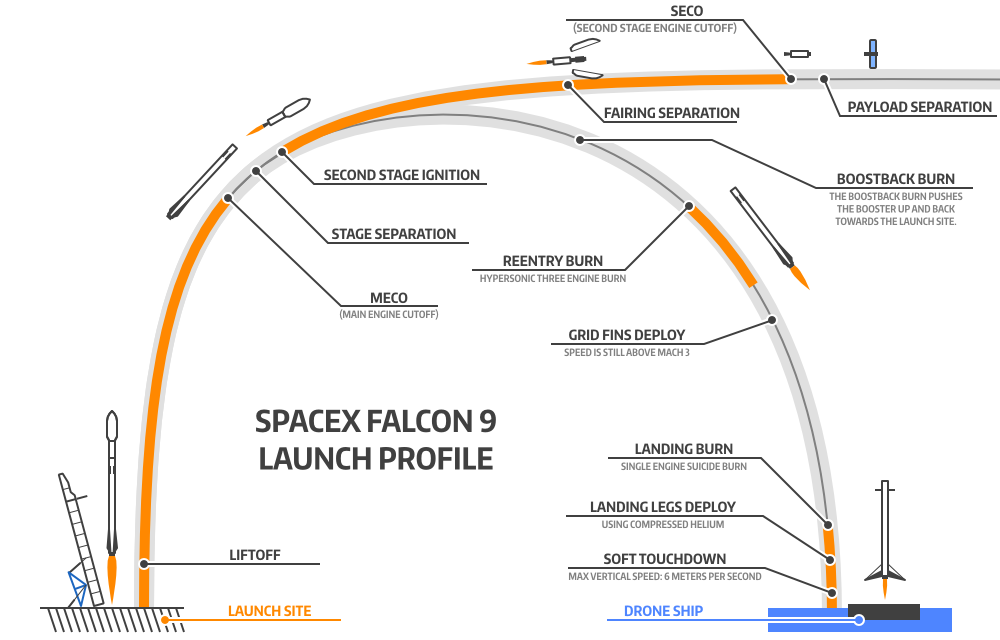
\includegraphics[width=\textwidth]{images/suicideburn}
\end{frame}
{
\usebackgroundtemplate{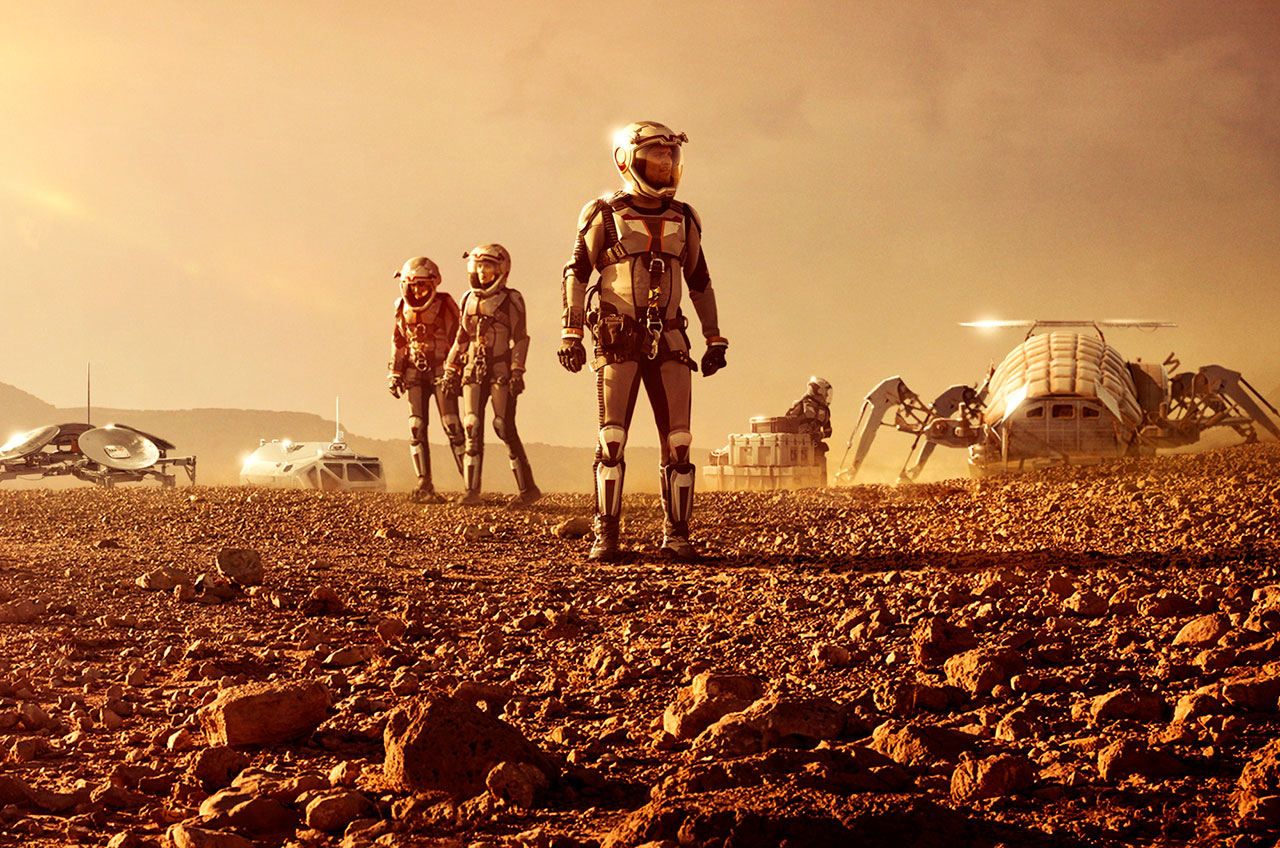
\includegraphics[height=\paperheight, keepaspectratio]{images/landed}}%
\begin{frame}[t]{}
\end{frame}
}
